\section{实验信息}

\subsection{简介}

\subsubsection{目标介绍}
本实验的目标是:训练一个智能体,让其在对地图不断的探索中学习移动策略,减少碰撞障碍物,以最少的步数从起点走到终点,并尽可能多的收集宝箱。
\subsubsection{地图介绍}

如\Cref{map},重返秘境地图中包含起点、终点、道路、障碍物、宝箱和加速增益,智能体在地图中没有全局视角。

\begin{figure}[H]
    \centering
    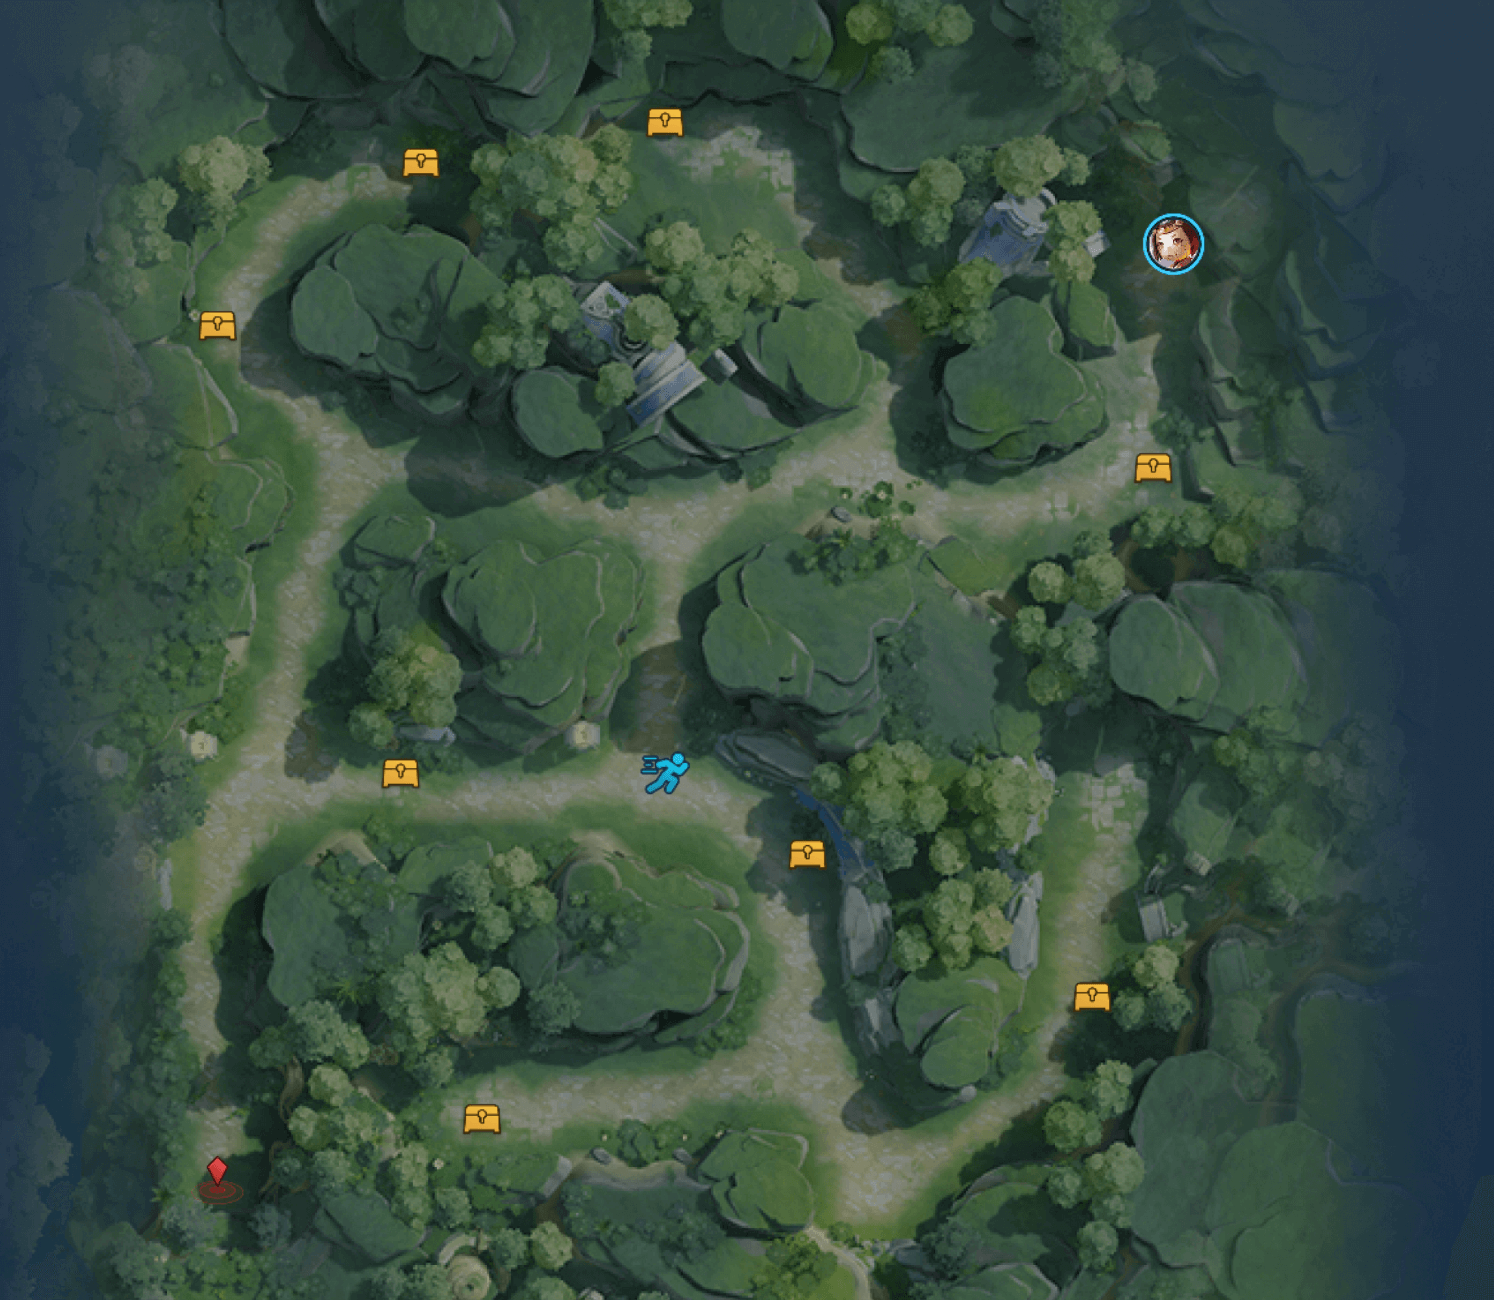
\includegraphics[width=0.8\linewidth]{pic/map.png}
    \caption{\zihao{-5} Map}
    \label{map}
\end{figure}

\Cref{elements} 中列举了地图中的所有元素。

\begin{table}[H]
    \begin{tabularx}{1\textwidth}{ l X } % | 表示垂直边框
        \hline % 水平边框
        \textbf{元素} & \textbf{说明}  \\
        \hline
        起点 & 任务开始时,智能体在起点出现。 \\
        终点 & 智能体的目的地,当智能体抵达终点时,任务结束。 \\
        道路 & 智能体可以在道路中有8个移动方向,智能体在执行一个动作后,会朝该动作表示方向持续移动3帧(1个step),然后在原地等待下一次动作指令。\\
        障碍物& 障碍物会阻挡智能体前进,当智能体在移动过程中遇到障碍物时,将紧贴障碍物边缘移动。有关智能体移动的详细介绍,请查看智能体移动及技能执行逻辑。\\
        宝箱 & 如果用户给任务配置了宝箱,则智能体可以通过拾取宝箱增加积分,每个宝箱获得100积分,地图中共有13个可配置宝箱的点位。可以通过配置宝箱的 数量 和 随机性 来调整环境的复杂度。 \\
        加速增益 & 在重返秘境地图中心存在一个加速增益,智能体可以通过拾取加速增益来提升自身的移动速度。在拾取加速增益后,移动速度提升 40\%,持续 10秒(约50个Step)。在增益结束后,智能体恢复默认速度。加速增益被拾取后会在 90秒(约454个Step) 后重新出现。 \\
        \hline
    \end{tabularx}

    \centering
    \caption{地图元素}
    \label{elements}
\end{table}

\subsubsection{智能体介绍}

\begin{enumerate}
    \item 视野域

    在重返秘境环境中,智能体只有局部视野:以智能体所在位置为中心,分别向“上、下、左、右”四个方向拓宽 25 格数的一个正方形观察域(size=51x51)。

    \item 技能

    智能体有 超级闪现 技能,使用该技能可以使智能体向指定方向位移8000。技能冷却时间 120秒(约606个Step)。
    当智能体使用超级闪现时,如果闪现的目的地在障碍物内(不在可移动的道路范围内),本次闪现技能将使用失败。
\end{enumerate}

\subsubsection{计分规则}

每一次游戏用户可以设定最大步数,如果智能体在最大步数内(包括最大步数)成功抵达终点,则判定任务成功,并按下方规则计算任务得分:

任务得分 = 终点得分 + 步数得分 + 宝箱得分

\begin{enumerate}
    \item 终点得分:到达终点即获得150分。
    \item 步数得分:(最大步数 - 完成步数) * 奖励系数0.2,完成步数是智能体抵达终点所用的步数。
    \item 宝箱得分:每获得一个宝箱,即可增加100分。
\end{enumerate}

注意:若在最大步数内没有走到终点,则判定为任务超时。超时任务的得分为0。

\subsection{环境介绍}

用户可以在 算法名称/train\_workflow.py 的 workflow 函数的参数中获取重返秘境环境 env:

\begin{adjustbox}{width=0.8\textwidth, center}
\begin{lstlisting}[language=Python]
def workflow(envs, agents, logger=None, monitor=None):
    env = envs[0] 
\end{lstlisting}
\end{adjustbox}

\quad

环境env有两个接口: reset 和 step,用户可以简单地通过以下方式来调用重返秘境环境:

\quad

\begin{adjustbox}{width=0.8\textwidth, center}
\begin{lstlisting}[language=Python]
obs = env.reset(usr_conf=usr_conf)
frame_no, _obs, score, terminated, truncated, env_info = env.step(act)
\end{lstlisting}
\end{adjustbox}

\subsubsection{环境配置}

用户可以在reset时传入一个usr\_conf来实现定制化的环境配置。
usr\_conf是一个字典类型,需要先定义一个 key 叫做 diy,diy的值包含一些键值对:

\begin{table}[H]
    \begin{tabularx}{1\textwidth}{ l l X } % | 表示垂直边框
        \hline % 水平边框
        \textbf{数据名} & \textbf{数据类型} & \textbf{说明}  \\
        \hline
        start & int & 起点编号,范围是[1,15],起点和终点不能重复 \\
        end & int & 终点编号, 范围是[1,15],起点和终点不能重复 \\
        treasure\_random & int & 是否生成随机宝箱,设置为1表示随机宝箱,设置为0表示固定宝箱,其他值非法 \\
        treasure\_num & int & 生成随机宝箱时的宝箱数量,仅在treasure\_random=1时生效,范围是 [1, 13] \\
        treasure\_id & list & 生成固定宝箱时的宝箱编号,仅在treasure\_random=0时生效,范围是 [1, 15],需要排除起点和终点编号,如果需要固定生成0个宝箱则传入[ ] \\
        max\_step & int & 单局最大步数,默认值为2000,无特殊需求不建议设置,过大的值会导致训练缓慢 \\
        talent\_type & int & 智能体技能,默认值为1,其他值非法 \\
        \hline
    \end{tabularx}

    \centering
    \caption{环境配置}
    \label{user-conf}
\end{table}

每个位置id对应的位置如\Cref{position}所示:

\begin{figure}[H]
    \centering
    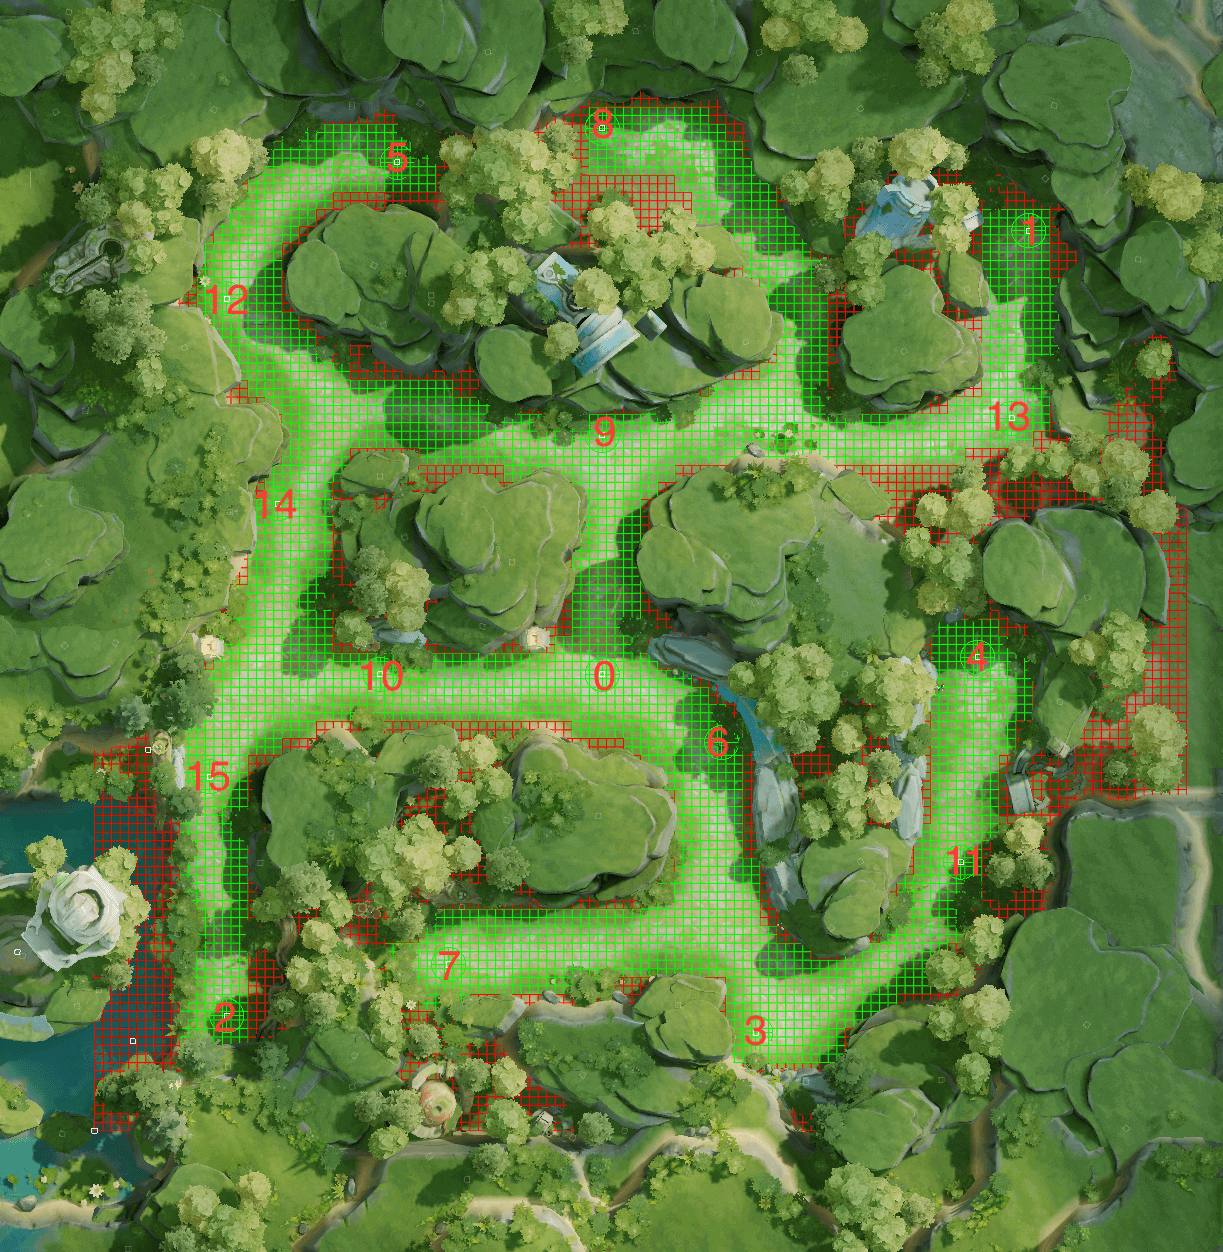
\includegraphics[width=0.8\linewidth]{pic/position.png}
    \caption{\zihao{-5} Position}
    \label{position}
\end{figure}

以下提供几个 usr\_conf 的设置实例:


\begin{enumerate}[label=例子\arabic*]
    \item 
\begin{lstlisting}[language=Python]
# 起点为2,终点为1,固定6个宝箱[4, 5, 6, 7, 8, 9]
usr_conf = {
    "diy": {
        "start": 2,
        "end": 1,
        "treasure_id": [4, 5, 6, 7, 8, 9],
        "treasure_random": 0,
        "talent_type": 1,
        "max_step": 2000,
    }
}
\end{lstlisting}

    \item 

\begin{lstlisting}[language=Python]
# 起点为2,终点为1,随机8个宝箱
usr_conf = {
  "diy": {
      "start": 2,
      "end": 1,
      "treasure_random": 1,
      "talent_type": 1,
      "treasure_num": 8,
      "max_step": 2000,
  }
}
\end{lstlisting}

    \item 

\begin{lstlisting}[language=Python]
# 起点为2,终点为1,固定0个宝箱
usr_conf = {
    "diy": {
        "start": 2,
        "end": 1,
        "treasure_id": [],
        "treasure_random": 0,
        "talent_type": 1,
        "max_step": 2000,
    }
}
\end{lstlisting}

\end{enumerate}

\subsection{环境信息}

用户调用env.step可以返回环境下一时刻的所有状态,以下 \Cref{environment-data} 是这些数据的描述,具体可以参考数据协议。


\begin{table}[H]
    \begin{tabularx}{1\textwidth}{l l X } % | 表示垂直边框
        \hline % 水平边框
        \textbf{数据名} & \textbf{数据类型} & \textbf{数据描述}  \\
        \hline
        frame\_no & int32 & 当前帧数 \\
        obs & <class 'custom\_pb2.Observation'> & 环境状态信息(观测信息) \\
        score & <class 'custom\_pb2.ScoreInfo'> & 得分信息 \\
        terminated & int32 & 表示游戏结束,即走到终点 \\
        truncated & int32 & 表示任务中断(超时或异常) \\
        env\_info & <class 'custom\_pb2.EnvInfo'> & 其他环境信息 \\
        \hline
    \end{tabularx}

    \centering
    \caption{环境数据}
    \label{environment-data}
\end{table}

用户调用env.reset可以返回环境的第一帧的状态,但仅包含观测空间obs。

\subsubsection{观测空间}

\Cref{measure-space} 返回的观测信息包含了当前环境的状态信息,具体包含属性feature和legal\_act,以下是这些数据的描述:

\begin{table}[H]
    \begin{tabularx}{1\textwidth}{l l X } % | 表示垂直边框
        \hline % 水平边框
        \textbf{数据名} & \textbf{数据类型} & \textbf{数据描述}  \\
        \hline
        norm\_pos&FloatPosition&归一化后的绝对坐标\\
        grid\_pos&Position&网格坐标\\
        start\_pos&RelativePosition&起点的相对位置\\
        end\_pos&RelativePosition&终点的相对位置\\
        buff\_pos&list(RelativePosition)&加速增益的相对位置\\
        treasure\_pos&RelativePosition&宝箱的相对位置\\
        obstacle\_map&list&周边障碍物信息\\
        memory\_map&list&周边记忆地图信息\\
        treasure\_map&list&周边宝箱信息\\
        end\_map&list&周边终点信息\\
        legal\_act&list&环境当前状态的可执行的动作        \\
        \hline
    \end{tabularx}

    \centering
    \caption{观测空间}
    \label{measure-space}
\end{table}

\subsubsection{位置信息}

以norm\_pos和grid\_pos为例,分别表示归一化后的绝对坐标和网格坐标,分别为FloatPosition类型和Position类型,norm\_pos由grid\_pos计算得到

\begin{lstlisting}[language=Python]
# FloatPosition的协议描述
message FloatPosition {
    float x = 1;                // x坐标
    float z = 2;                // z坐标
}
# Position的协议描述
message Position {
    int32 x = 1;                // x坐标
    int32 z = 2;                // z坐标
}
# 示例代码
pos = Position(x=100, z=100)
float_pos = FloatPosition(
        x=pos.x/64000,
        z=pos.z/64000,
)
\end{lstlisting}

\subsubsection{相对位置信息}

下面是对 \Cref{rel-pos} RelativePosition 详细的描述:

\begin{enumerate}
\item RelativePosition 表征的是英雄在任意位置时,物件的相对位置信息,比如方向,距离。其中:
\item RelativeDirection 通过枚举离散化表示方向信息。

RELATIVE\_DIRECTION\_NONE East NorthEast North NorthWest West SouthWest South SouthEast

\item RelativeDistance 通过枚举离散化表示距离信息。

RELATIVE\_DISTANCE\_NONE VerySmall Small Medium Large VeryLarge

\item path\_distance和grid\_distance是通过将地图网格化后计算出的从英雄当前格子到目标格子的网格路径最短距离,前者进行了离散化处理,后者进行了归一化处理。
\end{enumerate}


\begin{table}[H]
    \begin{tabularx}{1\textwidth}{l l X } % | 表示垂直边框
        \hline % 水平边框
        \textbf{RelativePosition} & \textbf{数据类型} & \textbf{数据描述}  \\
        \hline
        direction&RelativeDirection&相对方位(离散化)\\
        l2\_distance&RelativeDistance&L2距离(离散化)\\
        path\_distance&RelativeDistance&网格化后的最短路径距离(离散化)\\
        grid\_distance&float&网格化后的最短路径距离(归一化)        \\
        \hline
    \end{tabularx}

    \centering
    \caption{RelativePosition}
    \label{rel-pos}
\end{table}


\subsubsection{观测视野范围}

智能体观测到的地图范围是有限的,我们在观测空间中提供了智能体的视野域信息,即英雄周围的网格化后的局部信息。如 \Cref{scope} 所示:

\begin{figure}[H]
    \centering
    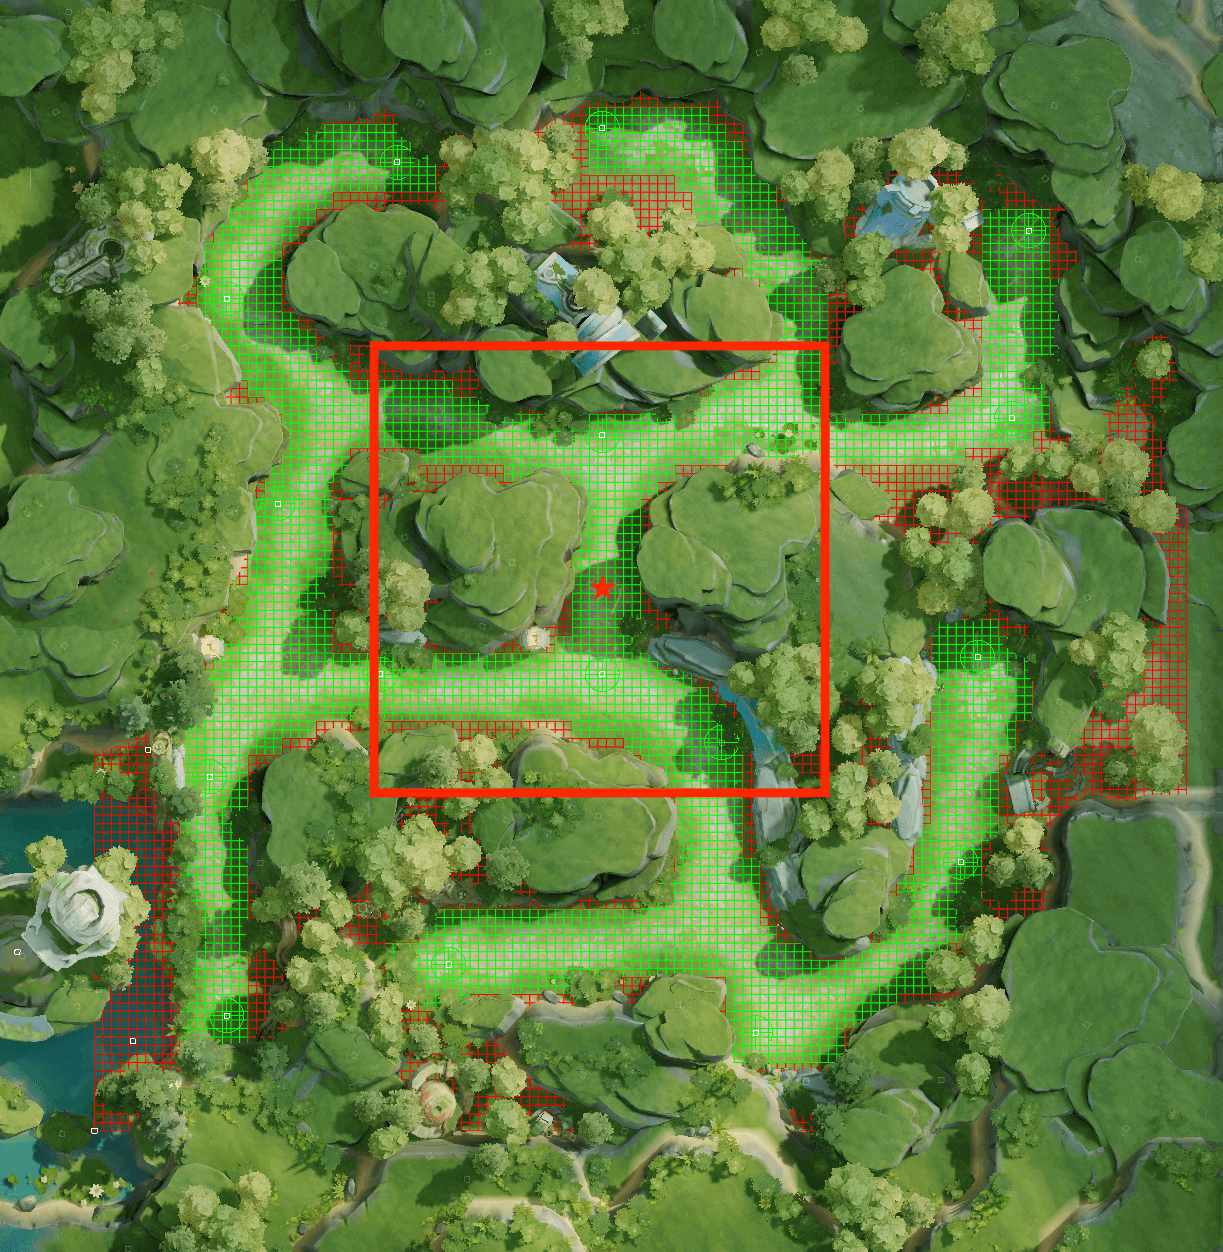
\includegraphics[width=0.8\linewidth]{pic/scope.png}
    \caption{\zihao{-5} 视野范围}
    \label{scope}
\end{figure}

\Cref{visible-scope} 视野域中会标注出障碍物、宝箱、终点以及记忆信息,分别存储在obstacle\_map、treasure\_map、end\_map、memory\_map四个向量中。


\begin{table}[H]
    \begin{tabularx}{1\textwidth}{l  X } % | 表示垂直边框
        \hline % 水平边框
        \textbf{向量名} & \textbf{说明}  \\
        \hline
        obstacle\_map&向量长度为2601,是51x51的矩阵视野域的一维展开,有阻挡的位置为0,无阻挡的位置为1。\\
        memory\_map&记录智能体探索每一个网格区域的次数,归一化到[0,1],初始化为0,每抵达一个网格,该网格坐标对应的值+0.2,最大为1。\\
        treasure\_map&标注宝箱的位置,有宝箱的位置为1,否则为0。\\
        end\_map&标注终点的位置,有终点的位置为1,否则为0。\\
        \hline
    \end{tabularx}

    \centering
    \caption{视野域}
    \label{visible-scope}
\end{table}

\subsection{动作空间}

重返秘境的动作空间分为两个部分:移动和技能,总的Action维度为16。env.step()传入的参数取值范围是[0, 15]


\subsubsection{移动}

移动使用的是8维离散化的动作空间,如\Cref{action-space}所示,将360度等分为8份,每45度角一个动作方向,以x轴正方向为起点,逆时针旋转。

\begin{figure}[H]
    \centering
    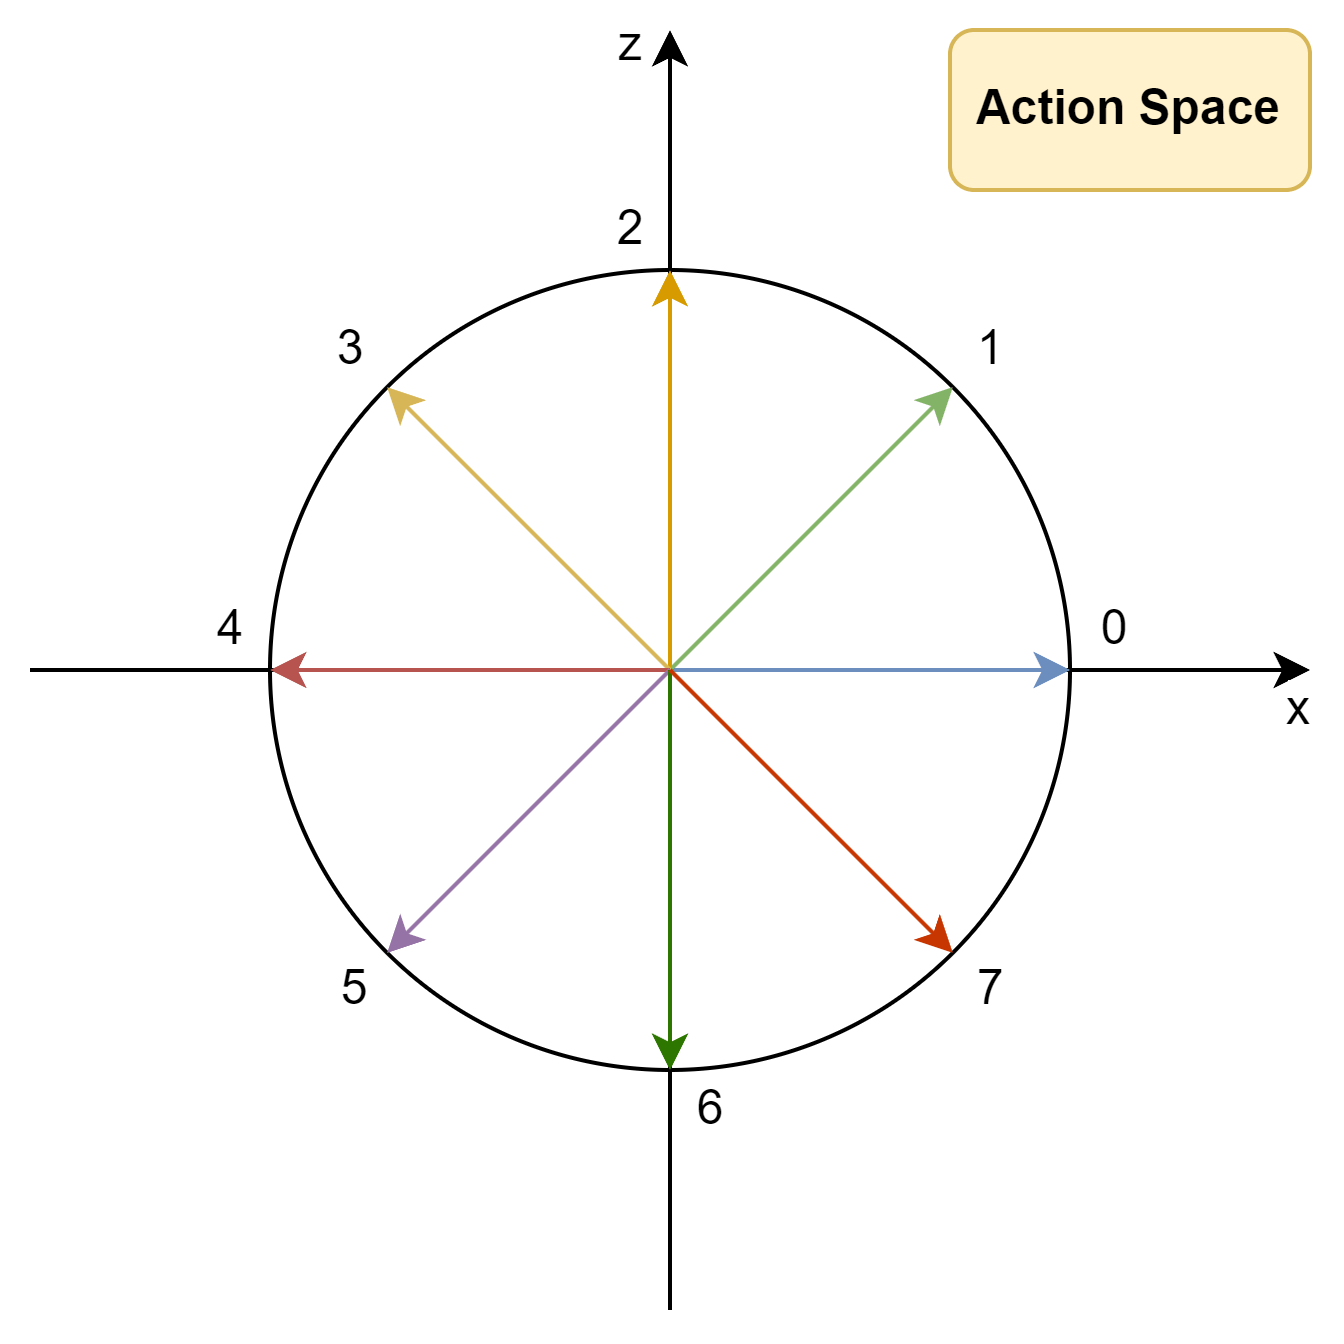
\includegraphics[width=0.8\linewidth]{pic/action-space.png}
    \caption{\zihao{-5} 移动}
    \label{action-space}
\end{figure}

对应关系如下:

\begin{lstlisting}[language=Python]
// 方向角,以x轴正方向为起始边
enum Direction {
    Angle_0 = 0;
    Angle_45 = 1;
    Angle_90 = 2;
    Angle_135 = 3;
    Angle_180 = 4;
    Angle_225 = 5;
    Angle_270 = 6;
    Angle_315 = 7;
}
\end{lstlisting}

我们将移动用一个8维的one-hot vector来表征,比如Direction = Angle\_90时,Action[0:8] = [0, 0, 1, 0, 0, 0, 0, 0]

\subsubsection{技能}

智能体有 超级闪现 技能,技能默认CD为120秒,闪现距离为8000,超级闪现的方向和移动方向一致。技能同样也是用一个8维的one-hot vector来表征,比如使用超级闪现且超级闪现方向Direction = Angle\_270时,Action[8:16] = [0, 0, 0, 0, 0, 0, 1, 0]。

\subsubsection{执行逻辑}


接下来介绍智能体移动和技能的执行逻辑。如\Cref{move}所示,在一次决策中,首先必须给智能体提供一个方向(8维的Direction),然后:

\begin{enumerate}
    \item  如果智能体执行移动动作,那么智能体会沿着该方向移动,一次预测(3帧)的移动距离大概为700,加速状态为1000。
    \begin{enumerate}
\item 移动方向上无障碍物:正常移动。
\item 移动方向上有障碍物:如下图白色箭头,移动方向的命令为Angle\_45=1, 实际执行时由于障碍物的阻挡,会沿着下方的白色箭头贴着障碍物的边缘移动。
    \end{enumerate}

    \item 如果智能体执行超级闪现动作,那么智能体会沿着该方向闪现,闪现距离为8000。

    \begin{enumerate}
\item 闪现方向上无障碍物:正常闪现,如下图的红色例子。
\item 闪现方向上有障碍物:
\item 闪现的目标位置无障碍物:穿墙闪现,如下图的蓝色箭头。
\item 闪现的目标位置有障碍物:闪现失败,原地不动,如下图的黄色箭头,英雄还是处于方块位置不动
    \end{enumerate}
\end{enumerate}


\begin{figure}[H]
    \centering
    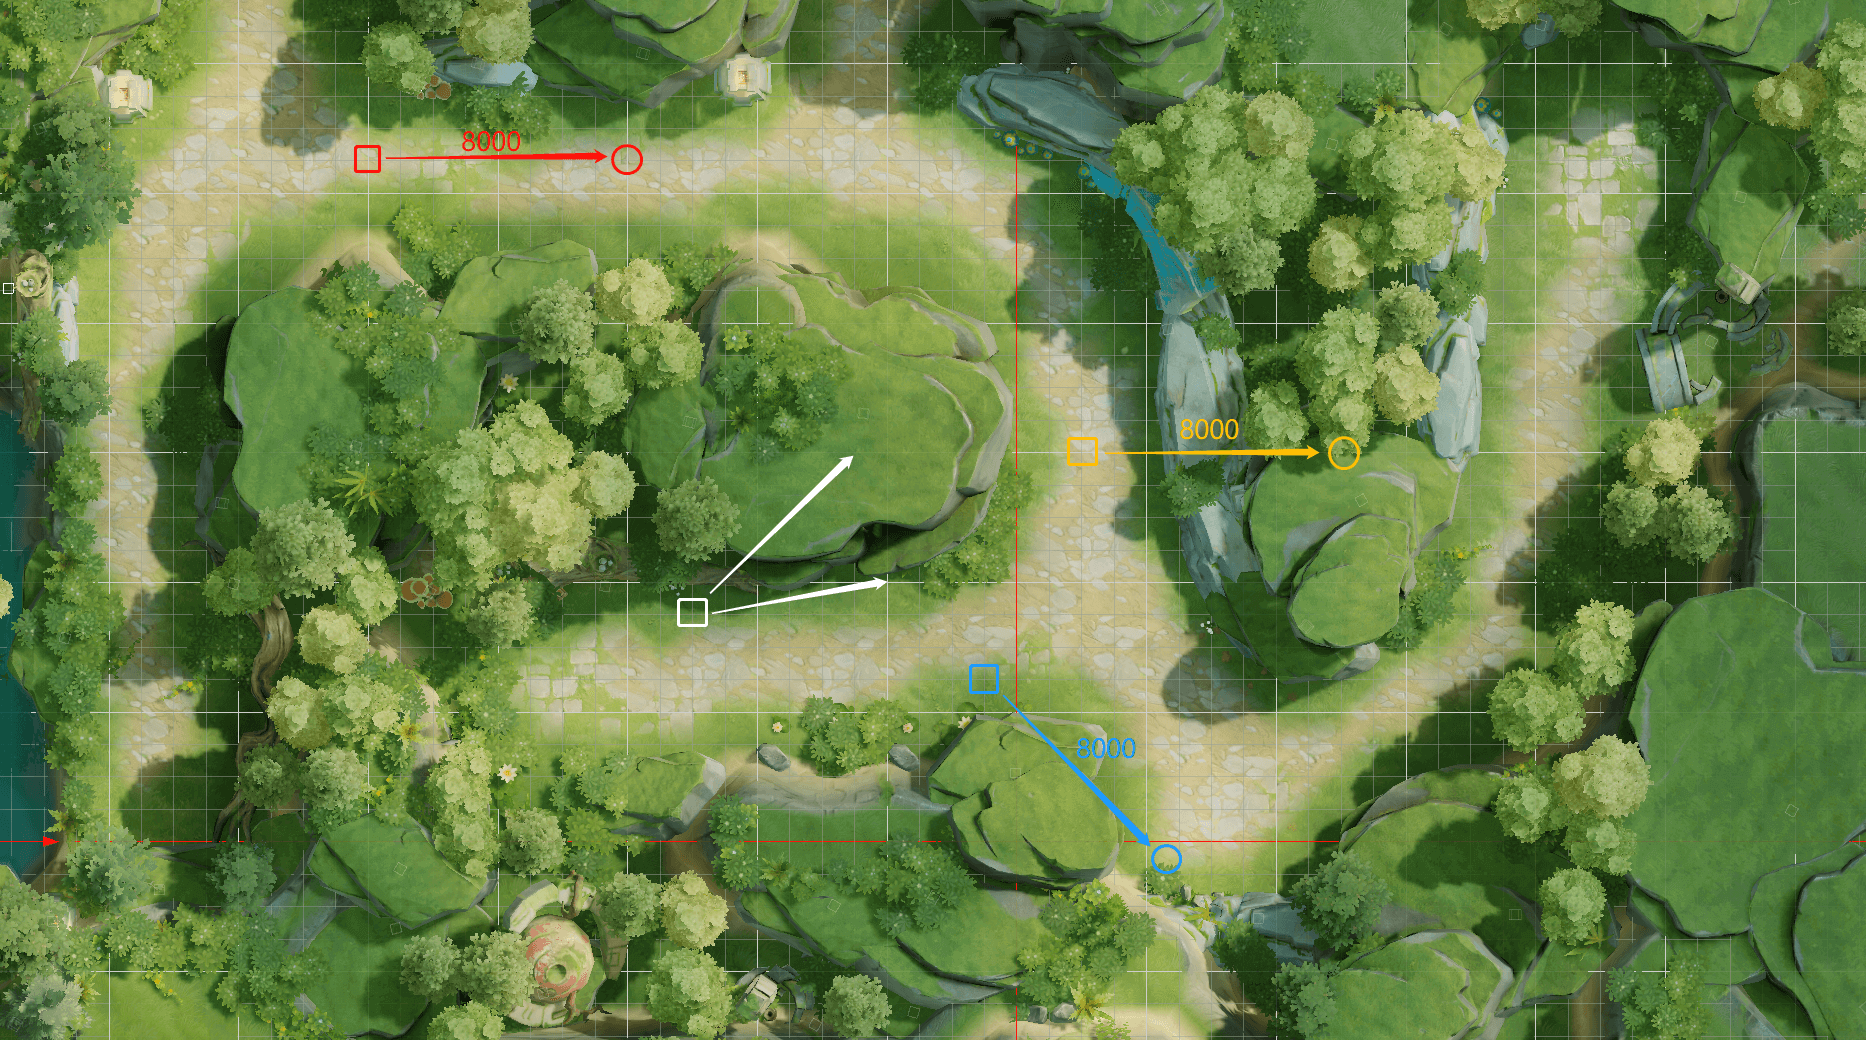
\includegraphics[width=0.8\linewidth]{pic/move.png}
    \caption{\zihao{-5} 移动}
    \label{move}
\end{figure}

补充说明:

\subsubsection{合法动作}

在环境中的某一时刻,不是所有的动作都可以被执行,因此我们需要向模型输入legal action,将网络结果进行掩码(masking)从而避免不符合规则的动作被输出。

在重返秘境中,超级闪现作为一个可执行的动作在冷却未结束时需要被避免使用,因此,在我们默认设置里将超级闪现是否可使用的信息作为legal action输入。

在默认设置里,legal\_action的输入为二维,第一维代表移动方向,第二维代表超级闪现方向。在超级闪现可以使用的时候移动和超级闪现都被允许预测,因此我们返还 [1, 1], 在超级闪现冷却时超级闪现不被允许输出,因此我们返还[1, 0]。在DQN算法的网络中输出16维的Q值信息,前八维对应八个可行走方向,后八维对应八个可超级闪现方向,第一维legal\_action对应前八维输出,第二维legal\_action对应后八维输出。

\subsection{得分信息}

env.step(act) 返回的 score 是在当前状态下执行动作 act 智能体所获得的分数,分数的计算详见计分规则。

\subsection{时间信息}

帧(frame)和步(step)存在一定映射关系。

帧是场景的一个时间单位,表示场景的一个完整更新周期。在每一帧中,场景的所有元素(如宝箱等)都会根据当前的状态和输入进行更新。

步是强化学习环境中的一个时间单位,表示智能体(agent)在环境中执行一个动作并接收反馈的过程。在每一步中,智能体选择一个动作,环境根据该动作更新状态,并返回新的状态、奖励和终止信号。

在本环境中,1个step由3个frame组成。这意味着每个动作对应一个步,在每一步中,智能体将在三个连续的帧中执行同一个动作。环境将在每一步结束后更新状态并返回反馈,场景只有在完成三帧后,环境状态才会返回一次状态的更新。

\begin{enumerate}
\item 步更新:在每一步中,智能体选择一个动作,环境更新状态并返回。
\item 帧更新:在一步中,场景进行三次帧更新,更新所有场景中对象的状态并渲染新的画面。
\end{enumerate}

帧(frame),步(step),现实时间秒(s)和现实时间毫秒(ms)的关系如下:

\begin{align*}
    1\,\text{frame} = 60 \,\text{ms} \\
    1\,\text{step} = 3\,\text{frame} \\
    1\,\text{s} = 1000\,\text{ms} \\
\end{align*}


注意 :由于运行环境的差异,每一帧的时间会在66毫秒上下浮动

\subsection{监控介绍}

在腾讯开悟平台的训练管理页面,提供了查看监控功能,点击后,即可在新标签页中打开监控面板,如下图所示。可以通过查看监控数据实时定位自己的训练进程,从而帮助大家评更快更准确的找到问题所在。

\subsubsection{监控面板介绍}

在监控面板中,包括 错误日志数量 和 监控指标图 两部分内容。

错误日志数量:在该模块中,可以看到训练过程中每个模块的错误日志数量。点击模块卡片可以进入日志详情页,查看该模块的错误日志信息。

监控指标图:在该模块中,可以看到四类数据指标,分别是basic(基础指标)、algorithm(算法指标)、env(环境指标)、diy(自定义指标)。

\begin{table}[H]
    \begin{tabularx}{1\textwidth}{ l X } % | 表示垂直边框
        \hline % 水平边框
        \textbf{指标分类} & \textbf{说明}  \\
        \hline
        basic&包括强化学习训练过程中的标准数据和资源使用数据。\\
        algorithm&和算法相关的数据指标,不同算法上报的指标可能会有所不同。\\
        env&和环境相关的数据指标,不同环境上报的指标不同。\\
        diy&用户自行上报的数据指标。\\
        \hline
    \end{tabularx}

    \centering
    \caption{监控面板}
    \label{monitor-dashboard}
\end{table}


\begin{enumerate}
    \item 基础指标

\begin{table}[H]
    \begin{tabularx}{1\textwidth}{ l X } % | 表示垂直边框
        \hline % 水平边框
        \textbf{指标名称} & \textbf{说明}  \\
        \hline
    train\_global\_step&训练的累计步数,即agent.learn的调用次数。取决于各算法的具体实现:DQN系列的算法从样本池中采样一次后调用agent.learn。\\
    predict\_succ\_cnt&采样预测的累计帧数,即agent.predict的调用次数。\\
    sample\_production\_and\_consumption\_ratio&等于训练步数除以采样预测的累计帧数。\\
    episode\_cnt&已经结束的任务个数。\\
    load\_model\_succ\_cnt&预测加载模型文件成功的次数,即调用agent.load\_model的调用次数。\\
    sample\_receive\_cnt&learner成功接收的样本数量。\\
        \hline
    \end{tabularx}
    \centering
    \caption{基础指标}
    \label{monitor-basic}
\end{table}


    \item 算法指标

\begin{table}[H]
    \begin{tabularx}{1\textwidth}{ l X } % | 表示垂直边框
        \hline % 水平边框
        \textbf{指标名称} & \textbf{说明}  \\
        \hline
        reward&累积回报,反应了智能体的能力,正常训练情况下指标应该是震荡向上。\\
        q\_value&target网络的Q值,一定程度反应Q值的稳定性。\\
        value\_loss&计算loss的标量值,反应训练的进程,正常情况下指标应该是逐渐接近于0。\\
        \hline
    \end{tabularx}
    \centering
    \caption{算法指标}
    \label{monitor-alg}
\end{table}

    \item 环境指标

\begin{table}[H]
    \begin{tabularx}{1\textwidth}{ l X } % | 表示垂直边框
        \hline % 水平边框
        \textbf{指标名称} & \textbf{说明}  \\
        \hline
        score & 该面板包含两个指标:total\_score:任务结束时的得分,若任务超时,则该局得分为0。treasure\_score:任务结束时收集到的宝箱奖励。\\
        steps & 该面板包含两个指标:max\_steps:任务设置的最大步数。finished\_steps:任务结束时所用的步数。若任务超时,则该局完成步数等于最大步数。\\
        treasure & 该面板包含两个指标:total\_treasures:任务设置的宝箱个数。collected\_treasures:任务结束时收集到的宝箱个数。\\
        treasure\_random & 宝箱是否随机。若为0则表示宝箱位置固定,若为1则表示宝箱位置随机。\\
        skill\_cnt & 技能使用次数。\\
        buff\_cnt & 加速增益拾取次数。\\
        \hline
    \end{tabularx}
    \centering
    \caption{环境指标}
    \label{monitor-env}
\end{table}

    \item diy(自定义指标)

    我们提供了五个自定义指标diy\_1至diy\_5以便用户可以上报自己想要监控的数据。

    \begin{figure}[H]
        \centering
        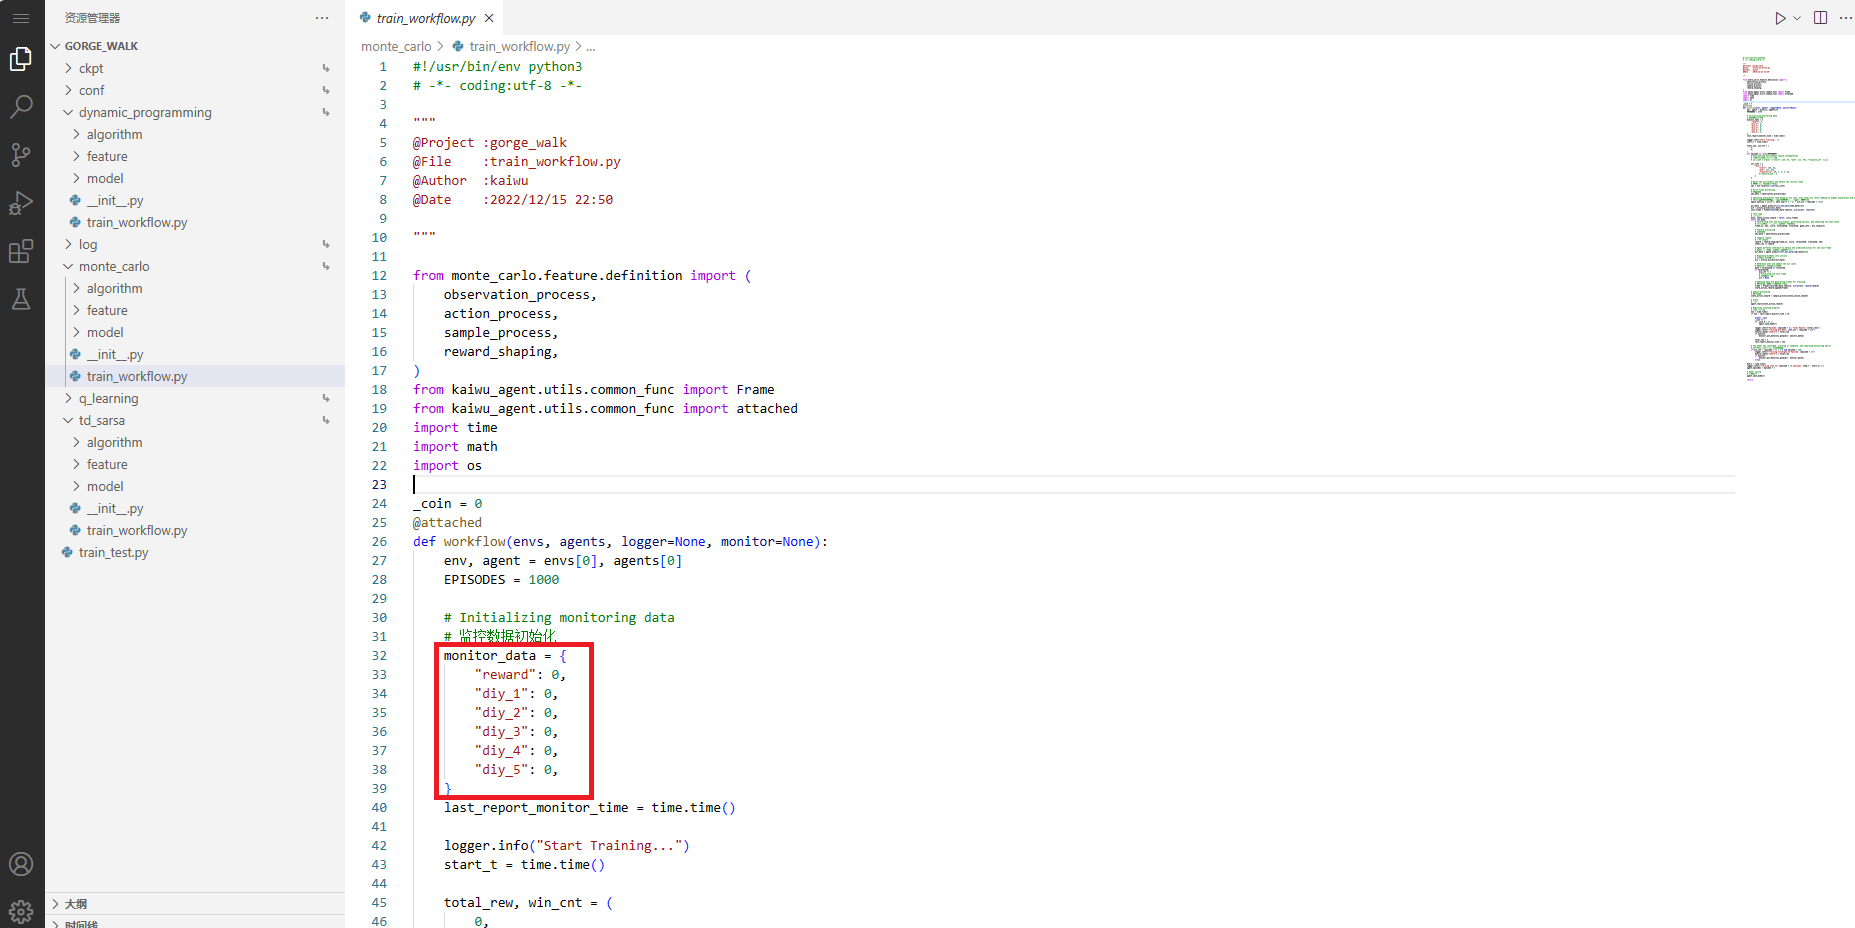
\includegraphics[width=1\linewidth]{pic/diy.png}
        \caption{\zihao{-5} 自定义指标}
        \label{diy}
    \end{figure}

\end{enumerate}

